\documentclass[11pt,a4paper,twoside]{book}
\linespread{1.3}

\usepackage[main=english,polish]{babel}

\usepackage[T1]{fontenc}
\usepackage[utf8]{inputenc}
% \usepackage[sfdefault,scaled=.95]{FiraSans}

\usepackage[lf]{Baskervaldx} % lining figures
\usepackage[bigdelims,vvarbb]{newtxmath} % math italic letters from nimbus Roman
\usepackage[cal=boondoxo]{mathalfa} % mathcal from STIX, unslanted a bit
\renewcommand*\oldstylenums[1]{\textosf{#1}}

\usepackage[table]{xcolor}
\definecolor{plum}{RGB}{150,95,119}
\definecolor{grafit}{RGB}{60,60,60}

\usepackage{amsmath,amsfonts}
% \usepackage{icomma}
\usepackage{textcomp}
\usepackage{gensymb}

\usepackage{graphicx}

\usepackage[left=3cm,right=2cm,top=2.5cm,bottom=2.5cm]{geometry}

\usepackage{fancyhdr}
\pagestyle{fancy}
\renewcommand{\headrulewidth}{0pt}
\renewcommand{\footrulewidth}{1.5pt}
\renewcommand{\footrule}{{\color{plum}%
			\vskip-\footruleskip\vskip-\footrulewidth
			\hrule width\headwidth height\footrulewidth\vskip\footruleskip}}

\fancyhead{}
\cfoot{}
\fancyfoot[LE, RO]{\thepage}

\renewcommand\labelitemi{\color{plum}{\tiny$\blacksquare$}}
\renewcommand\labelitemii{\color{plum}{\tiny$\square$}}
\renewcommand\labelitemiii{\color{plum}{\tiny$\bullet$}}

\usepackage{enumitem}
\setlist[itemize]{noitemsep, topsep=0pt, leftmargin=1cm, itemindent=0cm}

\usepackage{nowidow}
\widowpenalty=10000
\clubpenalty=10000
\brokenpenalty 10000
\sloppy

\usepackage[skip=4pt,indent=0cm,parfill=0pt]{parskip}

\usepackage{array}
\usepackage{multicol}
\usepackage{multirow}
\renewcommand*{\figurename}{Fig.}
\renewcommand*{\tablename}{Tab.}
\arrayrulecolor{plum}
\renewcommand\thefootnote{\textcolor{plum}{\arabic{footnote}}}
\usepackage[font={footnotesize},justification=centerlast]{caption}
\numberwithin{equation}{chapter}
\newcolumntype{M}[1]{>{\centering\arraybackslash}m{#1}}
\usepackage{subfig}

\usepackage{lipsum}

\let\lll=\relax

\usepackage[inkscapelatex=false]{svg}
\usepackage[version=4]{mhchem}
\usepackage{braket}
\usepackage{listings}

\textwidth=16cm
\textheight=24cm

\raggedbottom
\renewcommand{\arraystretch}{1.4}

\usepackage{catchfile}
\newcommand{\getenv}[2][]{%
  \CatchFileEdef{\temp}{"|kpsewhich --var-value #2"}{\endlinechar=-1}%
  \if\relax\detokenize{#1}\relax\temp\else\let#1\temp\fi}

\getenv[\INDEX]{INDEX}

\newcommand{\probP}{\text{I\kern-0.15em P}}
\newcommand{\thesistitle}{Influence of the reconstruction efficiency on the angular correlation functions in Run 3 software in ALICE.}
\newcommand{\thesistitlepl}{\begin{otherlanguage}{polish}
    Wpływ wydajności rekonstrukcji śladów cząstek na kątowe funkcje korelacyjne w oprogramowaniu Run 3 w eksperymencie ALICE.
\end{otherlanguage}}

\usepackage{hyperref}
\hypersetup{
	pdftitle = {\thesistitle},
	pdfauthor = {Dawid Karpiński},
	colorlinks,
	linktoc=page,
	linkcolor=plum,
	citecolor=plum,
	filecolor=plum,
	urlcolor=plum
}


\begin{document}

\setlength{\arrayrulewidth}{1pt}
\setlength{\jot}{12pt}
\setlength{\parskip}{0.6em}
\setlength{\parindent}{0em}
\setlength{\abovedisplayskip}{20pt}
\setlength{\belowdisplayskip}{30pt}
\setlength{\footskip}{40pt}

\pagestyle{empty}

\begin{titlepage}
	\begin{minipage}{\textwidth}
		\begin{center}
			
\includegraphics[scale=0.2]{img/WF_ENG} \\
			\vspace{1.5cm}
			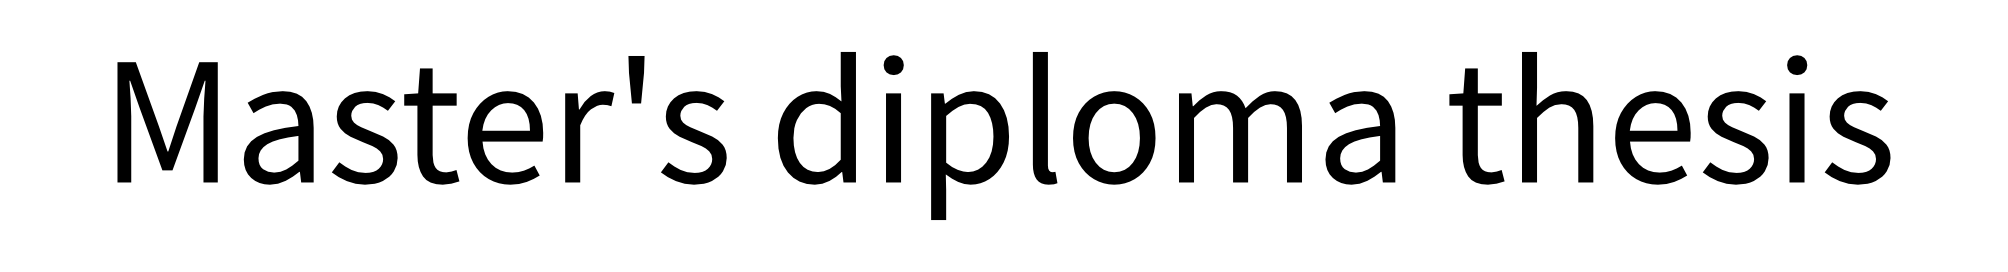
\includegraphics[width=0.7\textwidth]{img/mgr_en}
		\end{center}
	\end{minipage}

	\vspace{1.5cm}

	\begin{minipage}{\textwidth}
		\begin{center}
			{\large in the field of study Fizyka Techniczna \\
				and specialization EDMI}
		\end{center}
	\end{minipage}

	\vspace{1.5cm}

	\begin{minipage}{\textwidth}
		\begin{center}
			{\LARGE \thesistitle}
			\vspace{0.5cm}\\
			% TODO: thesis number
			{\large thesis number according to Faculty's thesis evidence: \{\}}
		\end{center}
	\end{minipage}

	\vspace{1.5cm}

	\begin{minipage}{\textwidth}
		\begin{center}
			{\LARGE Dawid Karpiński}
			\vspace{0.5cm}\\
			{\large student record book number: \INDEX}
		\end{center}
	\end{minipage}

	\vspace{1.5cm}

	\begin{minipage}{\textwidth}
		\begin{center}
			{\large supervisor: \\
				dr hab. inż. Małgorzata Janik}\\
			\vspace{0.5cm}
			{\large second supervisor: \\
				dr hab. inż. Łukasz Graczyk}
		\end{center}
	\end{minipage}%

	\vfill

	\begin{minipage}[b]{\textwidth}
		\begin{center}
			{\large WARSAW \the\year{}}
		\end{center}
	\end{minipage}
\end{titlepage}

\newpage
\mbox{ }

\newpage
{\Large Abstract}

{\color{plum}\rule[1pt]{\textwidth}{2pt}}

\textbf{Thesis title:} \thesistitle

% TODO: abstract

\vspace{0.025\textheight}
\textit{Keywords}\\
% TODO: keywords
\textit{}

\vfill

\begin{multicols}{2}
	\begin{flushleft}
		supervisor's signature
	\end{flushleft}
	\begin{flushright}
		student's signature
	\end{flushright}
\end{multicols}

\newpage
\mbox{ }

\newpage
{\Large Streszczenie}

{\color{plum}\rule[1pt]{\textwidth}{2pt}}

\textbf{Tytuł pracy:} \thesistitlepl

\vspace{0.025\textheight}
\textit{Słowa kluczowe:}\\
% TODO: slowa kluczowe
\textit{}

\vfill

\begin{multicols}{2}
	\begin{flushleft}
		podpis opiekuna naukowego
	\end{flushleft}
	\begin{flushright}
		podpis studenta
	\end{flushright}
\end{multicols}

\newpage
\mbox{ }

\tableofcontents
\addtocontents{toc}{\protect\thispagestyle{empty}}
\pagestyle{empty}

% -------

\chapter{Introduction}
\pagestyle{fancy}

\section{LHC and Run 3}

The \textbf{Large Hadron Collider} (LHC), located at the European Organization for Nuclear Research (CERN) near Geneva, Switzerland, stands as the world's largest particle accelerator. Created in 2008, it accelerates and collides particles, primarily protons and heavy ions (e.g., lead). These collisions produce a variety of subatomic particles, allowing us to test predictions of the Standard Model and search for new phenomena beyond it.

The collider has completed two successful periods of data collection, the first Run 1 (2010--2013), and the other Run 2 (2015--2018). The current operational phase, \textbf{Run 3}, began in 2022 following the second, long shutdown (LS2) \cite{lhc-upgrade}. After numerous upgrades, the LHC now features proton-proton collisions at a center-of-mass energy of 13.6 [TeV], an increase from the 13 [TeV] utilized in Run 2. This higher energy helps in further studies and improves measurement precision and analysis statistics.

\section{The ALICE experiment}

The acronym ALICE stands for \textbf{A Large Ion Collider Experiment}, one of four major experiments at the LHC. The detector enables the study of the quark-gluon plasma (QGP), a state with conditions resembling those a few millionths of a second after the Big Bang, before quarks and gluons combined to form protons and neutrons. Heavy ion nucleus-nucleus collisions can produce such a state. In the case of ALICE, the focus lies on lead-lead (Pb-Pb) collisions \cite{alice-cern}. The experiment also includes proton-nucleus collisions, as well as analysis of proton-proton collisions as reference data.

\section{Two-particle angular correlation function}

This thesis focuses on $\Delta\eta\Delta\varphi$ particle correlations derived from proton-proton collision data collected in the ALICE experiment.

% TODO: why these angles in particular?

\subsection{Pseudorapidity and azimuthal angle}

% TODO: angles, coordinate system

One can construct the angular correlation function using two quantities: pseudorapidity, $\eta$, and azimuthal angle, $\phi$. Both represent different aspects of a particle's trajectory in the detector.

First, the pseudorapidity, $\eta$, relates to the angle between the particle momentum $p$ and the beam axis as:
\begin{equation}
	\eta = -\ln\left[\tan\left(\frac{\theta}{2}\right)\right].
\end{equation}

The azimuthal angle on the other hand represents the angle between the $x$-axis and the projection of the momentum vector onto the $xy$-plane.

% TODO: image showing both angles

However, the analysis of two-particle correlation accounts for the differences between both angles, expressed as $\Delta\eta = \eta_1 - \eta_2$ and $\Delta\varphi = \varphi_1 - \varphi_2$.

\subsection{Angular correlation function}

To construct the $\Delta\eta\Delta\varphi$ correlation function, one first obtains the so-called \textbf{signal distribution}, $S(\Delta\eta, \Delta\varphi)$, by pairing every particle with every other particle, all within the same event.

Next, through the event mixing, in which pairs consist of particles from different events, one calculates the \textbf{background distribution}, $B(\Delta\eta, \Delta\varphi)$. This aids in eliminating any single-particle effects.

% TODO: write more why?

As the last step, one should normalize both distributions normalized by the corresponding numbers of pairs in the same events, $N_{\text{same}}$, and mixed events, $N_{\text{mixed}}$, respectively.

Finally, the formula for the angular correlation function takes the form:
\begin{equation}
	C(\Delta\eta, \Delta\varphi) = \frac{S(\Delta\eta, \Delta\varphi)}{N_{\text{same}}} \frac{N_{\text{mixed}}}{B(\Delta\eta, \Delta\varphi)}.
\end{equation}

\section{Correction procedure}

The correction procedure aims to mitigate biases, that arise during the actual experiment.

Obtaining the weights used for correction happens based on data collected through Monto Carlo simulations (MC for short). Generated collisions follow set parameters, producing many particles referred to as \textbf{MC truth}. Extracted directly from the event itself, these particles remain unaffected by any effects that might come e.g. from detectors. Furthermore, the tracks of the same particles run through detectors for reconstruction and classification, hence called \textbf{MC reconstructed}.

\subsection{Reconstruction efficiency}

\begin{figure}[ht]
	\centering
	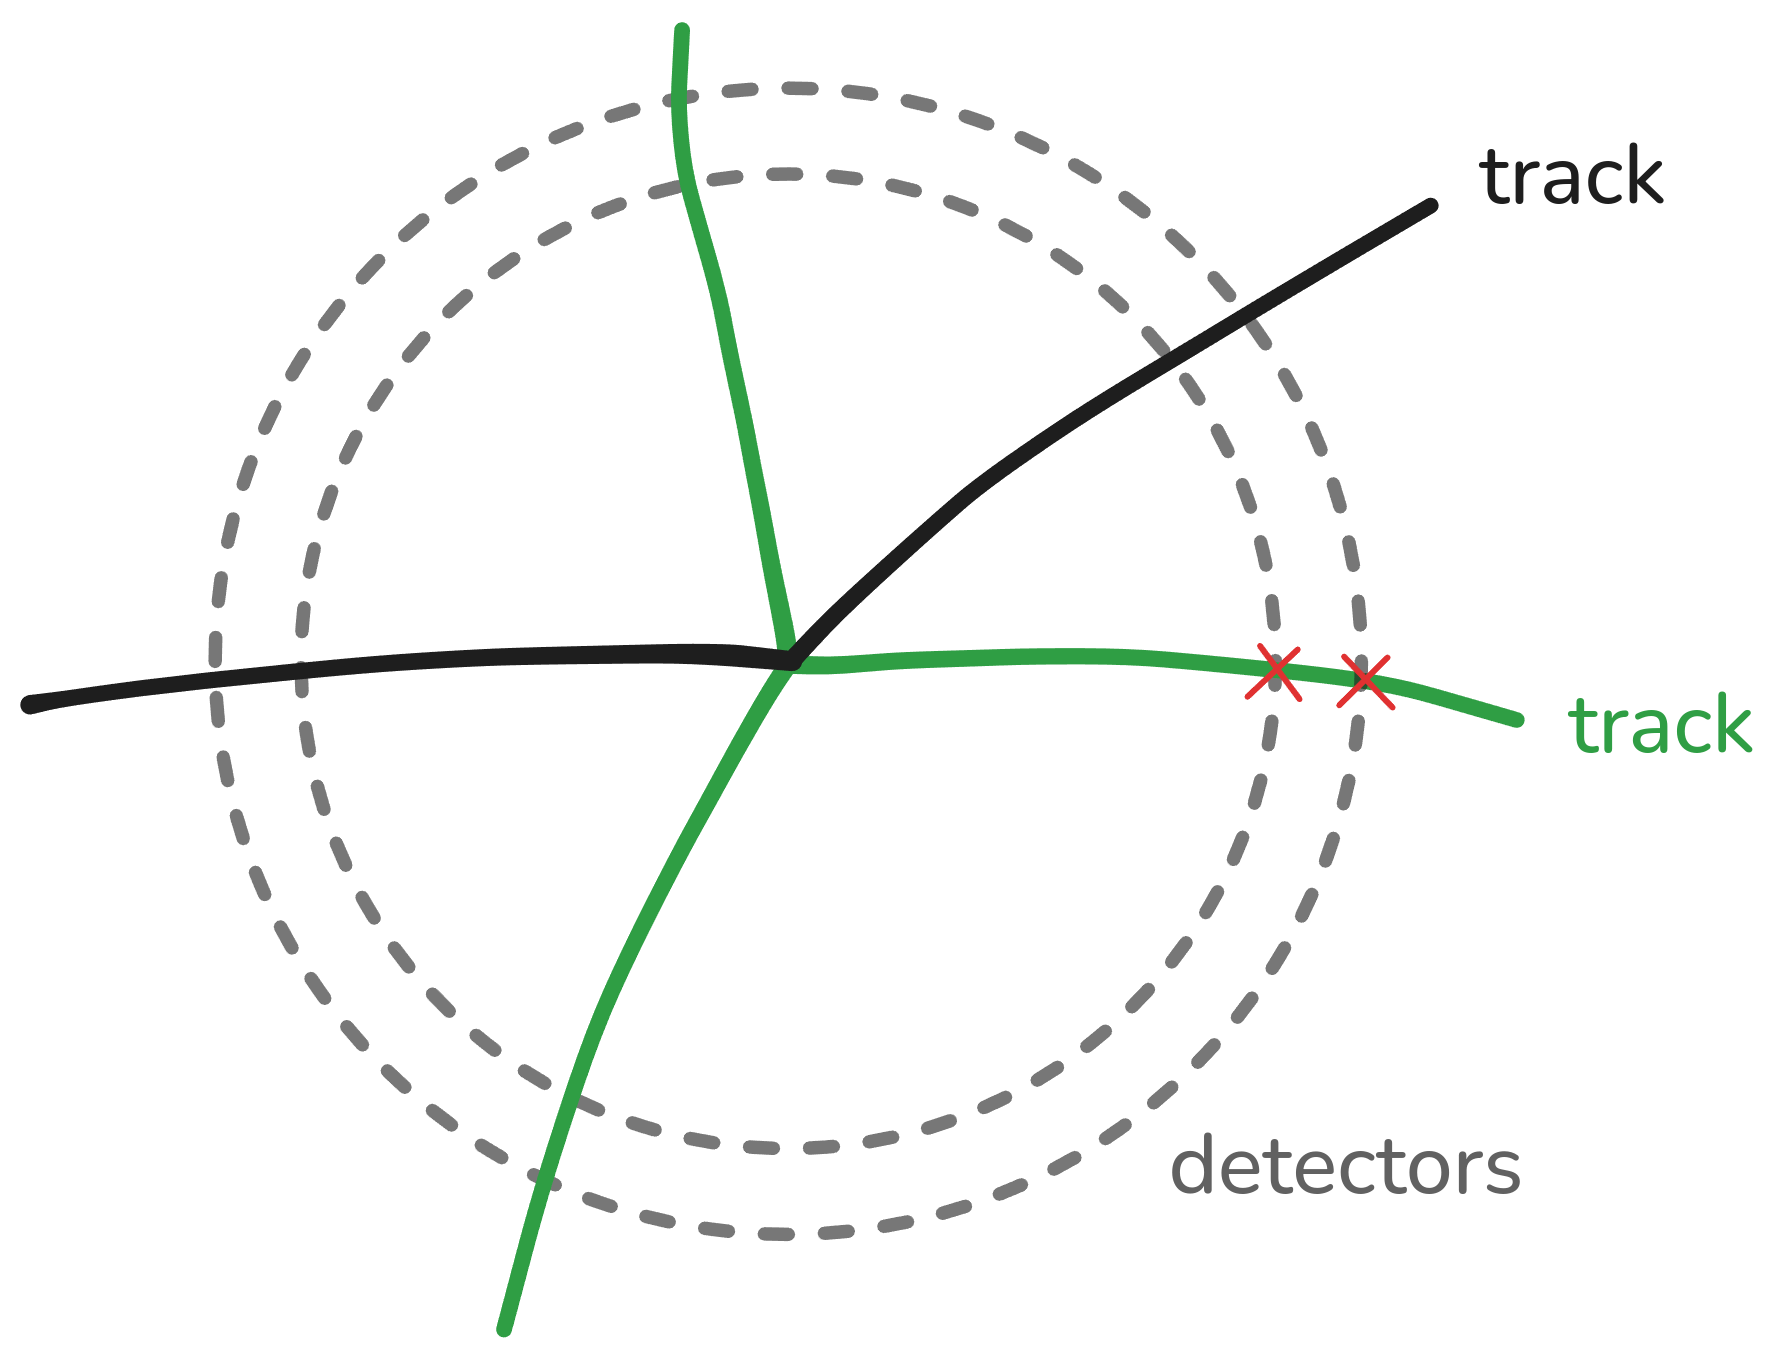
\includegraphics[width=0.6\textwidth]{img/efficiency.png}
	\caption{Tracks of simulated and reconstructed particles. Successful identification shown in green.}
	\label{fig:reco-truth-tracks}
\end{figure}

Therefore, calculation of reconstruction efficiency involves taking the ratio of the number of simulated (true) particles to the number of reconstructed particles:
\begin{equation}
	\varepsilon = \frac{N_{\text{recon.}}}{N_{\text{truth}}}.
\end{equation}

% TODO: transverse momentum, mc reco, mc truth, detection

\subsection{Secondary contamination}

However, ensuring the correct results in the efficiency calculations requires consideration of only the primary particles.

The secondary contamination, $C$, described as the ratio of the number of primary particles (such as protons, kaons, pions) over all recorded particles, can act as the correction factor to reconstruction efficiency. It ensures that the final weights base only on the expected particles.

% TODO: plot of hOrigin_MC, something with and without contamination ?

\subsection{Efficiency correction weights}

Having all the necessary quantities, mainly the efficiency histogram and secondary contamination, one can calculate the weights e.g. for each $p_T$ bin as:
\begin{equation}
	w(p_T) = \frac{1 - C(p_T)}{\varepsilon(p_T)}.
\end{equation}

% TODO: can be 2D

% correction factor added to correlation function

\section{Framework — O2 and O2Physics}


\cite{alice-o2}

\section{CCDB}

\section{GRID and HyperLoop}

% TODO: Highlight how the O2 framework utilizes HPC techniques, connecting to your "Podstawy High Performance Computing" course.

% -------

\chapter{Extending FemtoUniverse in the O2Physics framework}
\pagestyle{fancy}

% TODO: Installing and learning the O2 framework, and modifying the FemtoUniverse package to incorporate reconstruction efficiency corrections.
% TODO: Detail how you’ll use the O2 framework to handle big data challenges, such as efficiently processing Monte Carlo simulations and experimental data from LHC Run 3. Discuss data cleaning, transformation, and quality assurance (QA) steps.

\section{The old approach}

\section{The new additions}

\section{The final workflow for data correction}

% TODO: how does it help

% -------

\chapter{Data Analysis and Results}
\pagestyle{fancy}

\section{Reconstruction efficiency and purity}

% TODO: Calculating reconstruction efficiencies for pions, kaons, and protons using Monte Carlo data.

\section{MC closure}

\subsection{Correction influence on correlation functions}

% TODO: overall impact of corrections on the correlation functions

\subsection{Contamination factor impact}

\subsection{Efficiency influence in 1d vs. 2d}

\section{Correction on real data}

% TODO: comparison analysis MC vs. data, its impact


% TODO: Measuring angular correlation functions (in terms of relative pseudorapidity, Δη, and azimuthal angle, Δφ) with and without efficiency corrections.


% -------

\chapter{}
\pagestyle{fancy}

% -------

\bibliography{bib}
\bibliographystyle{unsrt}

\listoffigures
\listoftables

\appendix

\end{document}
